\documentclass[11pt,a4paper]{scrartcl}
\typearea{12}
\usepackage{graphicx}
\usepackage{pstricks}
\usepackage{listings}
\lstset{language=python}
\pagestyle{headings}
\markright{Computation Neuroscience - Lecture 5}
\begin{document}


\subsection*{The bucket-like equation for neurons}

We will now try to extend this bucket-like equation so that it applies
to neurons. First off $V$ is now voltage and $C$ will be replaced by
$c_m$, the capacitance of the membrane, the amount of electrical
charge that can be stored at the membrane is $C_mV$. The amount of
electrical charge is the analogue of the volume of water. 

The charge leak is a bit more complicated, because of the chemical
gradients, that is the effects of the differing levels of ions inside
and outside the cell along and their propensity to diffuse, the
voltage at which there is no leaking of charge is not zero, it is
$E_L=-70 $mV, roughly. This is an important aspect of how neurons
behave, and one we will encounter again looking at the Hodgkin-Huxley
equation: you might at first expect that if the voltage inside the
cell was, say, -60 mV then even if there was a high conductivity for
potassium at the membrane, the potassium ions would stay in the cell:
they are positive ions after all and so a negative voltage means the
electrical force is attracting them to the inside of the
cell. However, this isn't quite what happens, there is a high
concentration of potassium inside the cell and because of the random
motion of particles associated with temperature, these have a tendency
to diffuse, that is to increase the entropy of the situation by
spreading out. It takes a force to counteract this. This is the
reversal potential, the voltage required for zero current even if
there is some conductivity. The leak potential takes into account a
mixture of a reversal potential and the effect of the ion pumps.

$G$ is now $G_m$, a conductance, measuring the porousness of the
membrane to the flow of ions. The leak current is $G_m(V-E_L)$, as
above, we actually divide across by it, and write $R_m=1/G_m$, the
resistance. Finally, we write $\tau_m=C_m/G_m$ to get
\begin{equation}
\tau_m\frac{dV}{dt}=E_L-V+R_mI
\end{equation}
$I$ might end up being synaptic input, but traditionally we write the
equation to match the \textsl{in vivo} experiment where $I$ is an
injected current from an electrode, so we write $I_e$, \lq{}e\rq{} for
electrode.

This leaves out the possibility that there are other non-linear
changes in the currents through the membrane as $V$ changes. This is a
problem since there are other non-linear changes in the currents
through the membrane as $V$ changes. The equation above leaves these
out, in fact, the nonlinear effects are strongest for values of $V$
near where a spike is produced, so one approach is to use the linear
equation unless $V$ reaches a threshold value and then add a spike \lq{}by
hand\rq{}. This is the \textbf{leaky integrate and fire model}.

\begin{itemize}
\item $V$ satisfies
\begin{equation}
\tau_m\frac{dV}{dt}=E_L-V+R_mI_e
\end{equation}
\item If $V\ge V_T$ a spike is recorded and the voltage is set to $V_R$.
\end{itemize}

This model is easy to solve; if $I_e$ is constant we have already
solved it above up to messing around with constants. If $I_e$ is not
constant it may still be possible to solve the equation, but in any
case the equation can be solved numerically on a computer. Basically
you divide time up into small steps, assume $I_e$ is constant for each
small step and use the analytic constant-input equation to get from
one time step to another. Alternatively the equation can be solved
using a numerical approach to solving differential equations, such as
the Euler method, or Runge Kutta, or, as mentioned when discussing the
bucket equations, by using the constant-input current solution to
evolve across small time steps. An example in given in Fig.~\ref{v_i_f}.

\begin{figure}
\begin{center}
% GNUPLOT: LaTeX picture with Postscript
\begingroup
  \makeatletter
  \providecommand\color[2][]{%
    \GenericError{(gnuplot) \space\space\space\@spaces}{%
      Package color not loaded in conjunction with
      terminal option `colourtext'%
    }{See the gnuplot documentation for explanation.%
    }{Either use 'blacktext' in gnuplot or load the package
      color.sty in LaTeX.}%
    \renewcommand\color[2][]{}%
  }%
  \providecommand\includegraphics[2][]{%
    \GenericError{(gnuplot) \space\space\space\@spaces}{%
      Package graphicx or graphics not loaded%
    }{See the gnuplot documentation for explanation.%
    }{The gnuplot epslatex terminal needs graphicx.sty or graphics.sty.}%
    \renewcommand\includegraphics[2][]{}%
  }%
  \providecommand\rotatebox[2]{#2}%
  \@ifundefined{ifGPcolor}{%
    \newif\ifGPcolor
    \GPcolorfalse
  }{}%
  \@ifundefined{ifGPblacktext}{%
    \newif\ifGPblacktext
    \GPblacktexttrue
  }{}%
  % define a \g@addto@macro without @ in the name:
  \let\gplgaddtomacro\g@addto@macro
  % define empty templates for all commands taking text:
  \gdef\gplbacktext{}%
  \gdef\gplfronttext{}%
  \makeatother
  \ifGPblacktext
    % no textcolor at all
    \def\colorrgb#1{}%
    \def\colorgray#1{}%
  \else
    % gray or color?
    \ifGPcolor
      \def\colorrgb#1{\color[rgb]{#1}}%
      \def\colorgray#1{\color[gray]{#1}}%
      \expandafter\def\csname LTw\endcsname{\color{white}}%
      \expandafter\def\csname LTb\endcsname{\color{black}}%
      \expandafter\def\csname LTa\endcsname{\color{black}}%
      \expandafter\def\csname LT0\endcsname{\color[rgb]{1,0,0}}%
      \expandafter\def\csname LT1\endcsname{\color[rgb]{0,1,0}}%
      \expandafter\def\csname LT2\endcsname{\color[rgb]{0,0,1}}%
      \expandafter\def\csname LT3\endcsname{\color[rgb]{1,0,1}}%
      \expandafter\def\csname LT4\endcsname{\color[rgb]{0,1,1}}%
      \expandafter\def\csname LT5\endcsname{\color[rgb]{1,1,0}}%
      \expandafter\def\csname LT6\endcsname{\color[rgb]{0,0,0}}%
      \expandafter\def\csname LT7\endcsname{\color[rgb]{1,0.3,0}}%
      \expandafter\def\csname LT8\endcsname{\color[rgb]{0.5,0.5,0.5}}%
    \else
      % gray
      \def\colorrgb#1{\color{black}}%
      \def\colorgray#1{\color[gray]{#1}}%
      \expandafter\def\csname LTw\endcsname{\color{white}}%
      \expandafter\def\csname LTb\endcsname{\color{black}}%
      \expandafter\def\csname LTa\endcsname{\color{black}}%
      \expandafter\def\csname LT0\endcsname{\color{black}}%
      \expandafter\def\csname LT1\endcsname{\color{black}}%
      \expandafter\def\csname LT2\endcsname{\color{black}}%
      \expandafter\def\csname LT3\endcsname{\color{black}}%
      \expandafter\def\csname LT4\endcsname{\color{black}}%
      \expandafter\def\csname LT5\endcsname{\color{black}}%
      \expandafter\def\csname LT6\endcsname{\color{black}}%
      \expandafter\def\csname LT7\endcsname{\color{black}}%
      \expandafter\def\csname LT8\endcsname{\color{black}}%
    \fi
  \fi
  \setlength{\unitlength}{0.0500bp}%
  \begin{picture}(7200.00,5040.00)%
    \gplgaddtomacro\gplbacktext{%
      \csname LTb\endcsname%
      \put(594,440){\makebox(0,0)[r]{\strut{}-70}}%
      \put(594,922){\makebox(0,0)[r]{\strut{}-60}}%
      \put(594,1403){\makebox(0,0)[r]{\strut{}-50}}%
      \put(594,1885){\makebox(0,0)[r]{\strut{}-40}}%
      \put(594,2367){\makebox(0,0)[r]{\strut{}-30}}%
      \put(594,2848){\makebox(0,0)[r]{\strut{}-20}}%
      \put(594,3330){\makebox(0,0)[r]{\strut{}-10}}%
      \put(594,3812){\makebox(0,0)[r]{\strut{} 0}}%
      \put(594,4293){\makebox(0,0)[r]{\strut{} 10}}%
      \put(594,4775){\makebox(0,0)[r]{\strut{} 20}}%
      \put(726,220){\makebox(0,0){\strut{} 0}}%
      \put(1941,220){\makebox(0,0){\strut{} 20}}%
      \put(3157,220){\makebox(0,0){\strut{} 40}}%
      \put(4372,220){\makebox(0,0){\strut{} 60}}%
      \put(5588,220){\makebox(0,0){\strut{} 80}}%
      \put(6803,220){\makebox(0,0){\strut{} 100}}%
    }%
    \gplgaddtomacro\gplfronttext{%
      \csname LTb\endcsname%
      \put(2178,4602){\makebox(0,0)[r]{\strut{} $R_mI_e=16$ mV}}%
      \csname LTb\endcsname%
      \put(2178,4382){\makebox(0,0)[r]{\strut{} $R_mI_e=12$ mV}}%
      \put(4000,0){\makebox(0,0)[r]{\strut{} $t$ (ms)}}%
      \put(0,3000){\makebox(0,0)[r]{\strut{} $V$ (mV)}}%
    }%
    \gplbacktext
    \put(0,0){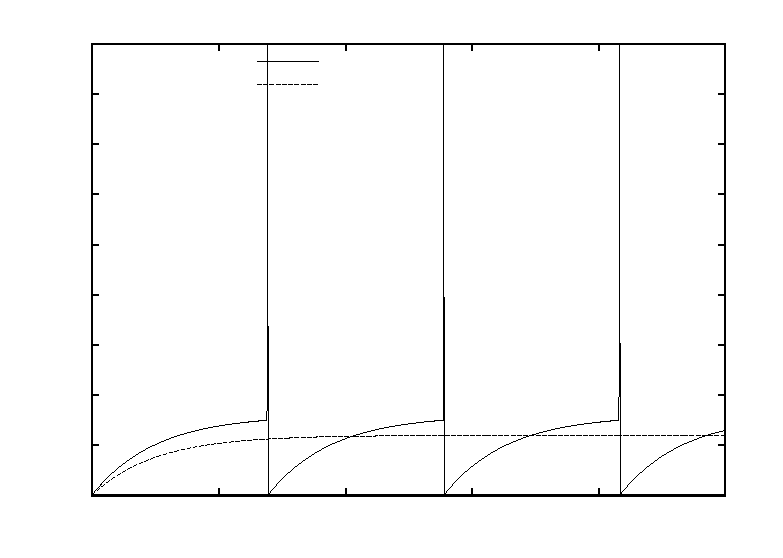
\includegraphics{v_i_f}}%
    \gplfronttext
  \end{picture}%
\endgroup

\end{center}
\caption{An integrate and fire neuron with different inputs. For
  $R_mI=12 $mV the voltage relaxes towards the equilibrium value
  $V=E_L+R_mI_e=-58$ mV. It never reaches the threshold value of
  $V_T=-55 $mV. For $R_mI=16$ mV the voltage reaches threshold and so
  there is a spike; the spike is added by hand, in this case by
  setting $V$ to $20$ mV for one time step. The voltage is then
  reset. Here $\tau_m=10$ mS.\label{v_i_f}}
\end{figure}

\end{document}

